\documentclass{beamer}
\mode<presentation>
\usepackage[orientation=landscape,size=a0,scale=1.4]{beamerposter}
\usetheme{AnnArbor}
\usepackage{siunitx}
\usepackage{wrapfig}
\title{Improving Nb\textsubscript{3}Sn Cavity Performance Using Mechanical Polishing}%
\author[shortname]{\large Eric Viklund \inst{1, 2} \and David Burk \inst{2} \and David N. Seidman \inst{1} \and Sam Posen \inst{2}}
\institute[shortinst]{\large \inst{1} Department of Materials Science and Engineering, Northwestern University \newline \inst{2} Fermi National Accelerator Laboratory}
\date{\today}%
\begin{document}%
    \begin{frame}{}
        \maketitle
        \begin{columns}[t]
            \begin{column}{0.32\linewidth}
                \begin{block}{\label{sec:introduction}Introduction}
                    Superconducting radiofrequency (SRF) cavities are essential components for providing the electric fields required to accelerate charged particles in particle accelerators. SRF cavities coated with a layer of Nb\textsubscript{3}Sn can reach up to 100~MV/m of accelerating field in theory. However, in practice surface roughness and other defects limit Nb\textsubscript{3}Sn SRF cavity performance. Centrifugal barrel polishing (CBP) is a proven technique for mechanically polishing Nb SRF cavities to nanometer scale smoothness. Here, we apply this technique to a Nb\textsubscript{3}Sn coated, 1.3~GHz, TESLA geometry SRF cavity, and see an improvement in the accelerating gradient. To show the evolution of the surface during CBP, we polish Nb\textsubscript{3}Sn samples using a special coupon cavity, which can simulate accurate polishing conditions. The samples show a very low surface roughness after 8 hours of polishing with only a few hundred nanometers of material removal.
                \end{block}
                \begin{block}{\label{sec:backgroundinformation}Background Information}
                    \begin{columns}[t]
                        \begin{column}{0.45\columnwidth}
                            \begin{itemize}
                                \item Centrifugal Barrel Polishing (CBP) is a technique used to polish niobium cavities without using toxic chemicals such as HF.
                                \item CBP uses a custom built tumbling machine that can fit up to 9-cell size cavities, and can accelerate the polishing media against the cavity surface with up to 6g of force.
                                \item An alumina nanoparticle suspension is used as the abrasive material. Felt cubes are added to push the abrasives against the cavity surface.
                            \end{itemize}  
                        \end{column}
                        \begin{column}{0.45\columnwidth}
                            \begin{figure}[t]%
                                \centering%
                                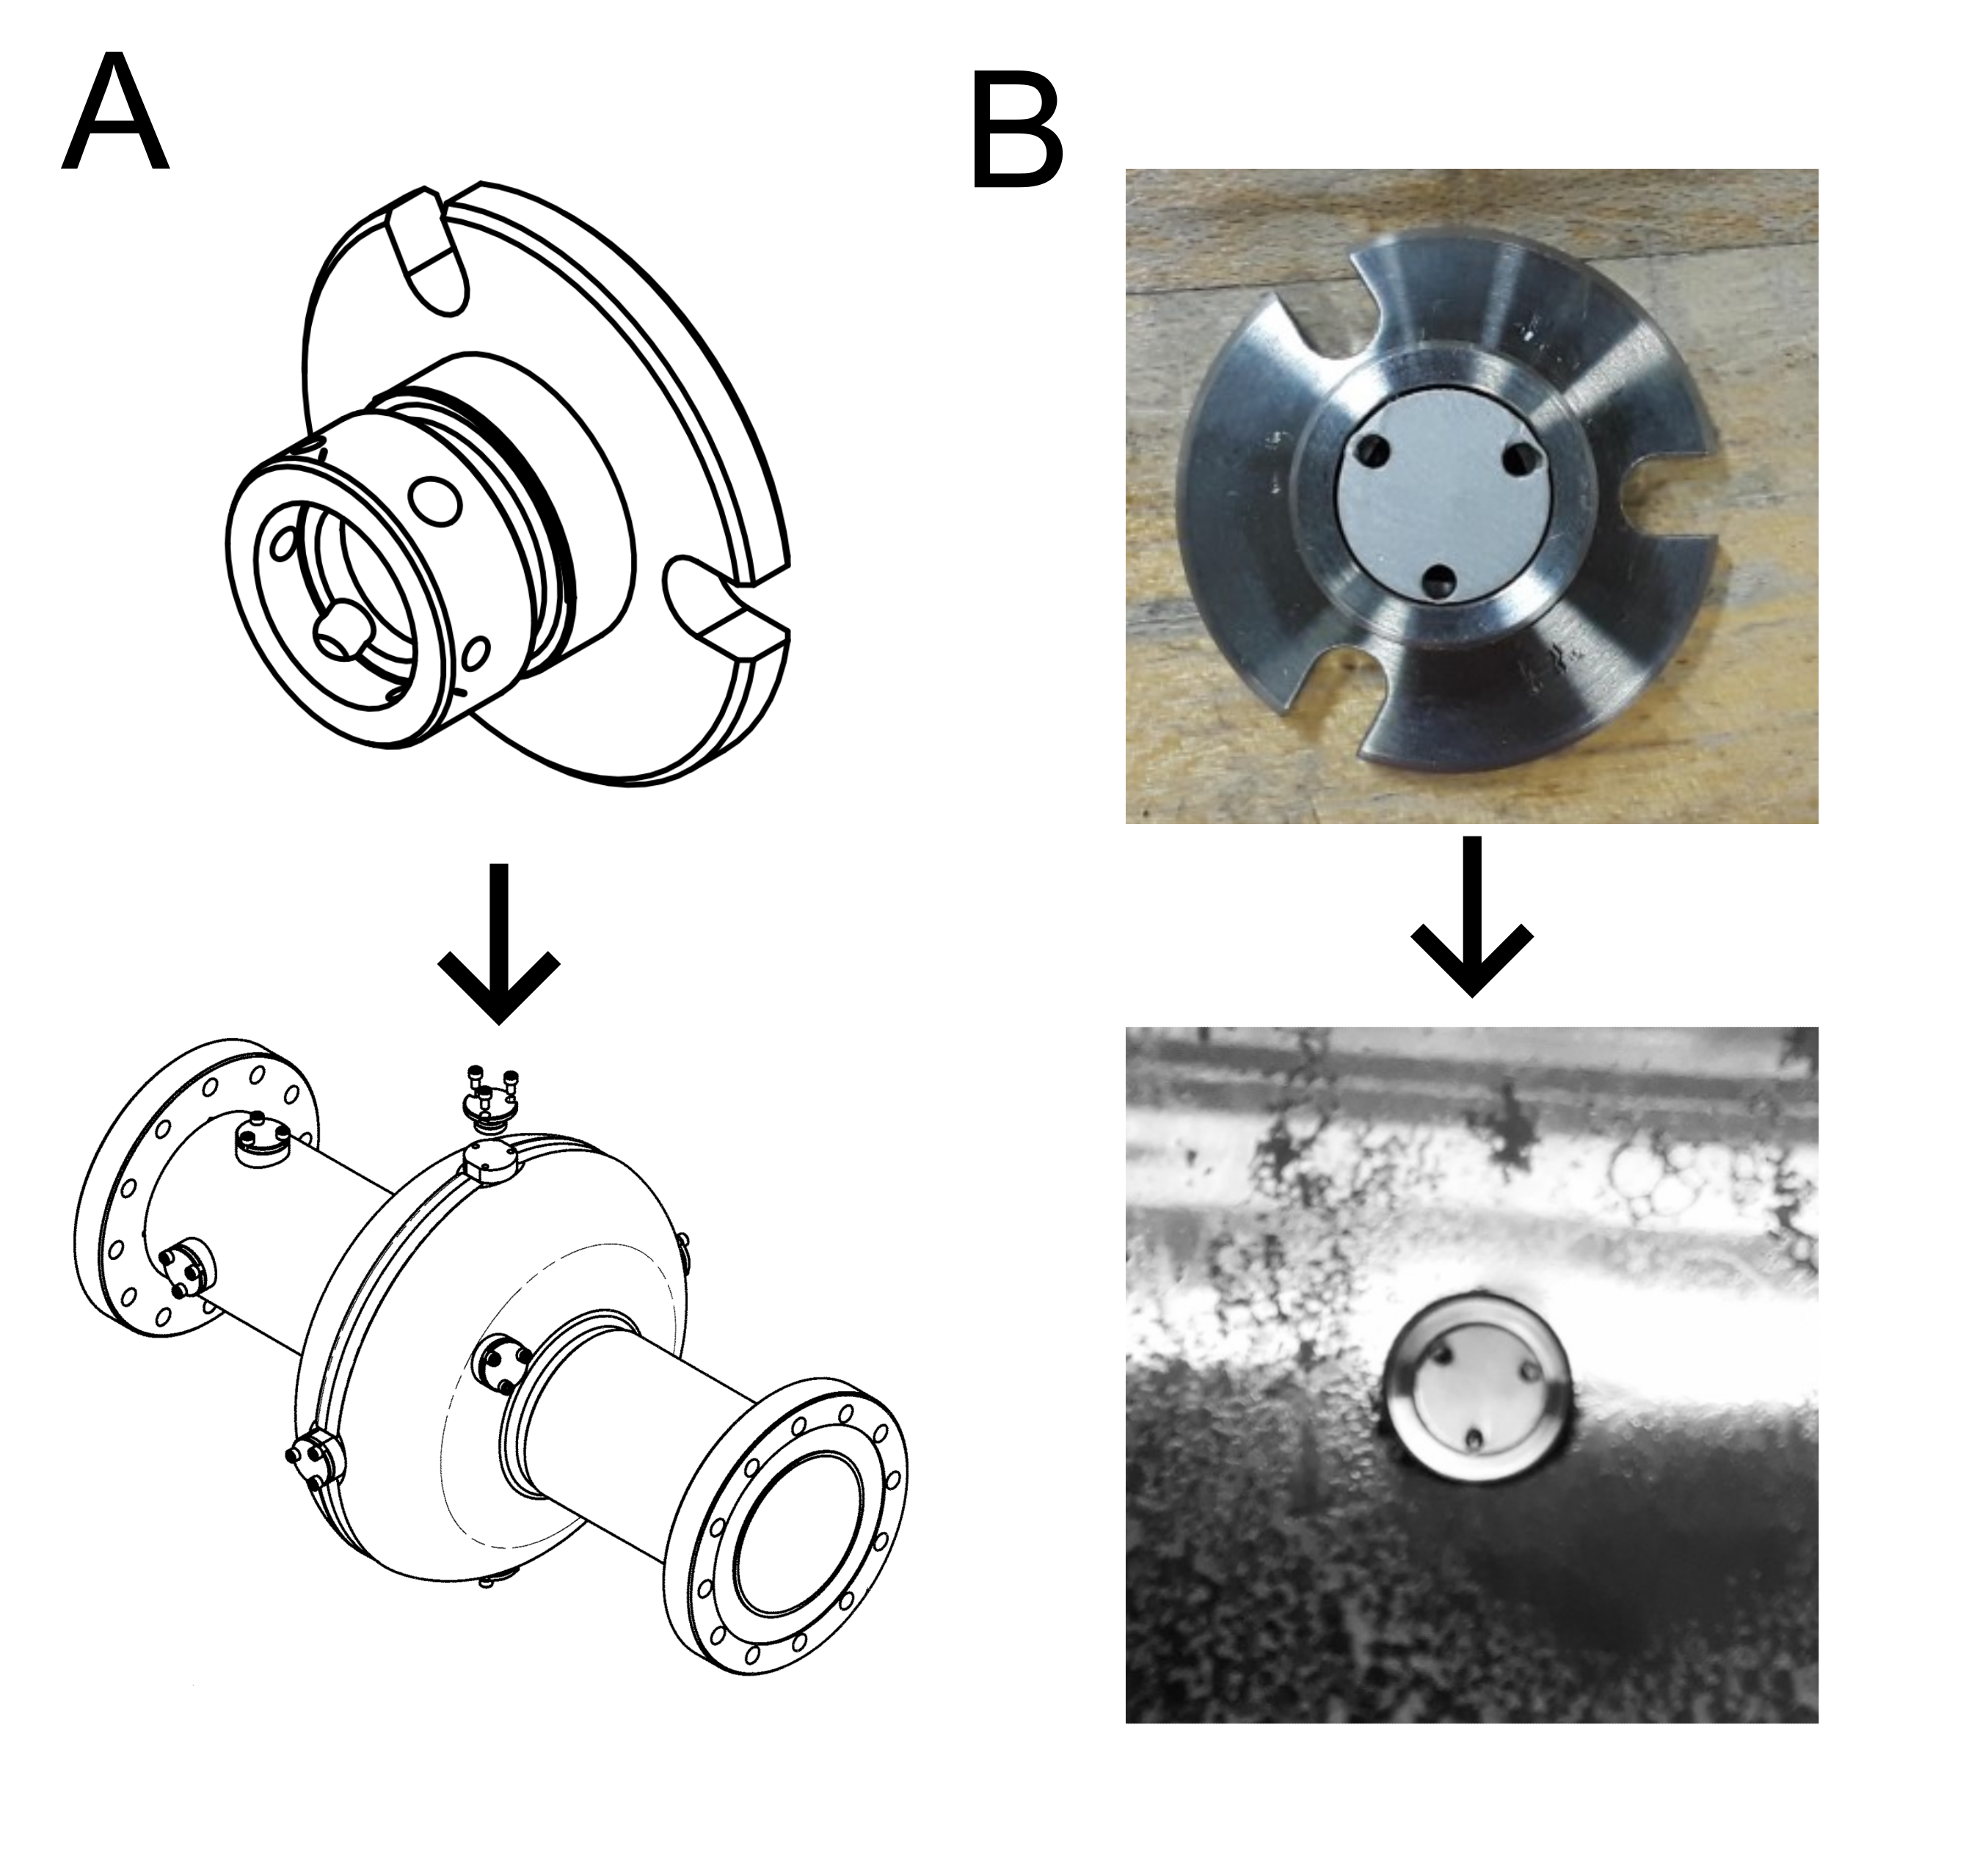
\includegraphics[width=\columnwidth]{../doc/figs/Coupon_Cavity.png}%
                                \caption{(A) A schematic of the coupon cavity and the sample holder used to polish the Nb\textsubscript{3}Sn coated samples. The sample holder can hold 1~cm diameter disks by clamping the sides of the sample with set screws. (B) Pictures of the sample holder sitting outside the coupon cavity and with a sample mounted as seen from the inside of the coupon cavity.}%
                                \label{fig:couponcavity}%
                            \end{figure}
                        \end{column}
                    \end{columns}
                \end{block}
            \end{column}
            \begin{column}{0.32\linewidth}    
                \begin{block}{\label{sec:samplestudy}Sample Study}
                    \begin{wrapfigure}{R}{0.3\columnwidth}
                        \centering
                        \includegraphics[width=0.25\columnwidth]{../doc/figs/Optical_Surface_Profiles.png}
                        \caption[width=0.25\columnwidth]{\label{fig:opticalsurfaceprofiles}Surface height maps of Nb\textsubscript{3}Sn samples mechanically polished for different lengths of time ranging from 2 to 8~hours compared to the initial state of the Nb\textsubscript{3}Sn coating.}
                        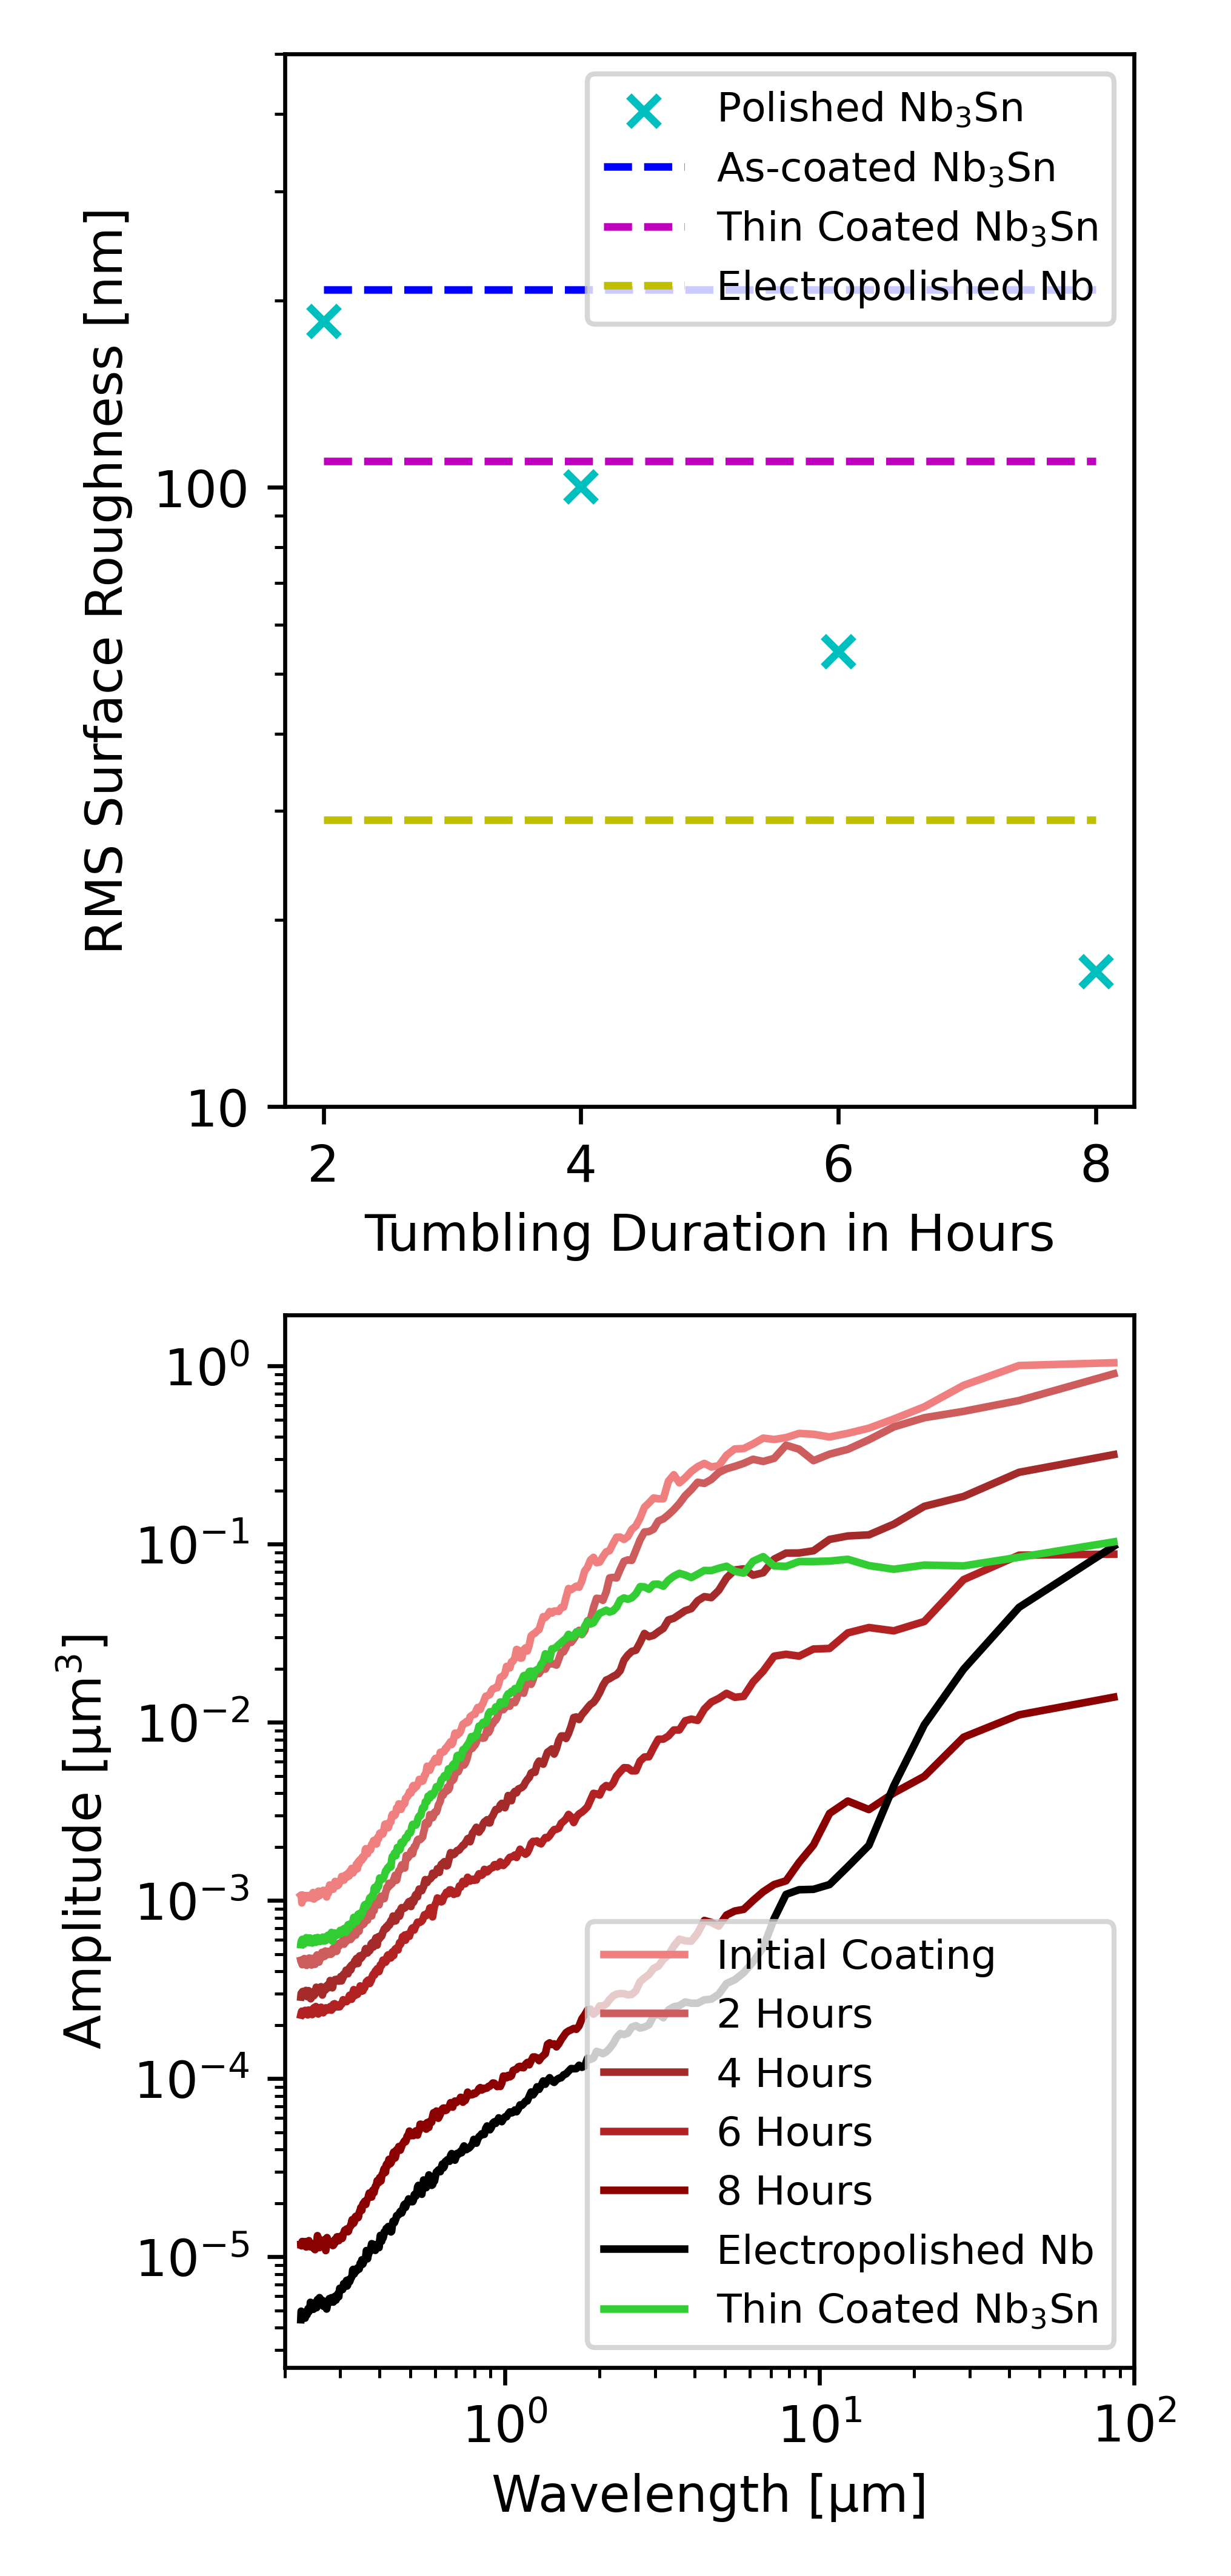
\includegraphics[width=0.25\columnwidth]{../doc/figs/Surface_Roughness_Graph.png}
                        \caption[width=0.25\columnwidth]{\label{fig:surfaceroughnessgraph}Surface roughness of Nb\textsubscript{3}Sn samples mechanically polished for different lengths of time calculated from the surface height maps (top). The power spectral density (PSD) of the surface profile after different amounts of tumbling as well as the PSD of electropolished Nb and a thinly coated Nb\textsubscript{3}Sn film.}
                    \end{wrapfigure}
                    Since Nb\textsubscript{3}Sn is a relatively unexplored material, there are no established polishing parameters or abrasive materials to achieve a good surface finish. To allow for rapid iteration and microscopy surface analysis, we first perform polishing experiments on Nb\textsubscript{3}Sn samples. To evaluate the performance of CBP, the surface roughness of the polished samples is measured using con-focal laser microscopy and the surface is analyzed using scanning and transmission electron microscopy (SEM and TEM). The material removal rate is measured using focused ion-beam tomography.
                    \begin{itemize}                        
                        \item A coupon cavity is used to test the centrifugal barrel polishing method on Nb\textsubscript{3}Sn samples in a realistic environment. The samples sit flush with the inside surface of the coupon cavity, where they experience identical polishing conditions to a real cavity surface.
                        \item The Nb\textsubscript{3}Sn samples and Nb\textsubscript{3}Sn cavity used in this study were coated at Fermilab in a high-vacuum furnace.
                        \item The surface roughness of the polished samples is measured using confocal laser microscopy, and the surface is analyzed using scanning and transmission electron microscopy (SEM and TEM). 
                        \item The removal rate of different abrasive materials has been measured using focused ion-beam tomography.
                        \item The smoothness of the samples improves as longer polishing is applied. Material is preferentially removed from the highest point on the surface, causing the sharp peaks on the surface to be removed quickly while valleys in the surface are left untouched. This is different from chemical polishing methods, which preferentially smooth areas with high curvature.
                        \item After 6~hours of polishing, the surface roughness is comparable to the surface roughness of the well-performing, thinly coated Nb\textsubscript{3}Sn coatings created at Fermilab. After 8~hours of polishing, the surface roughness is comparable to a typical niobium surface after EP.
                    \end{itemize}
                \end{block}
            \end{column}
            \begin{column}{0.32\textwidth}
                \begin{block}{\label{sec:cavitycbp}Polishing a Nb\textsubscript{3}Sn Cavity Using CBP}
                    \begin{columns}
                        \begin{column}{0.45\columnwidth}
                            \begin{figure}[t]
                                \centering
                                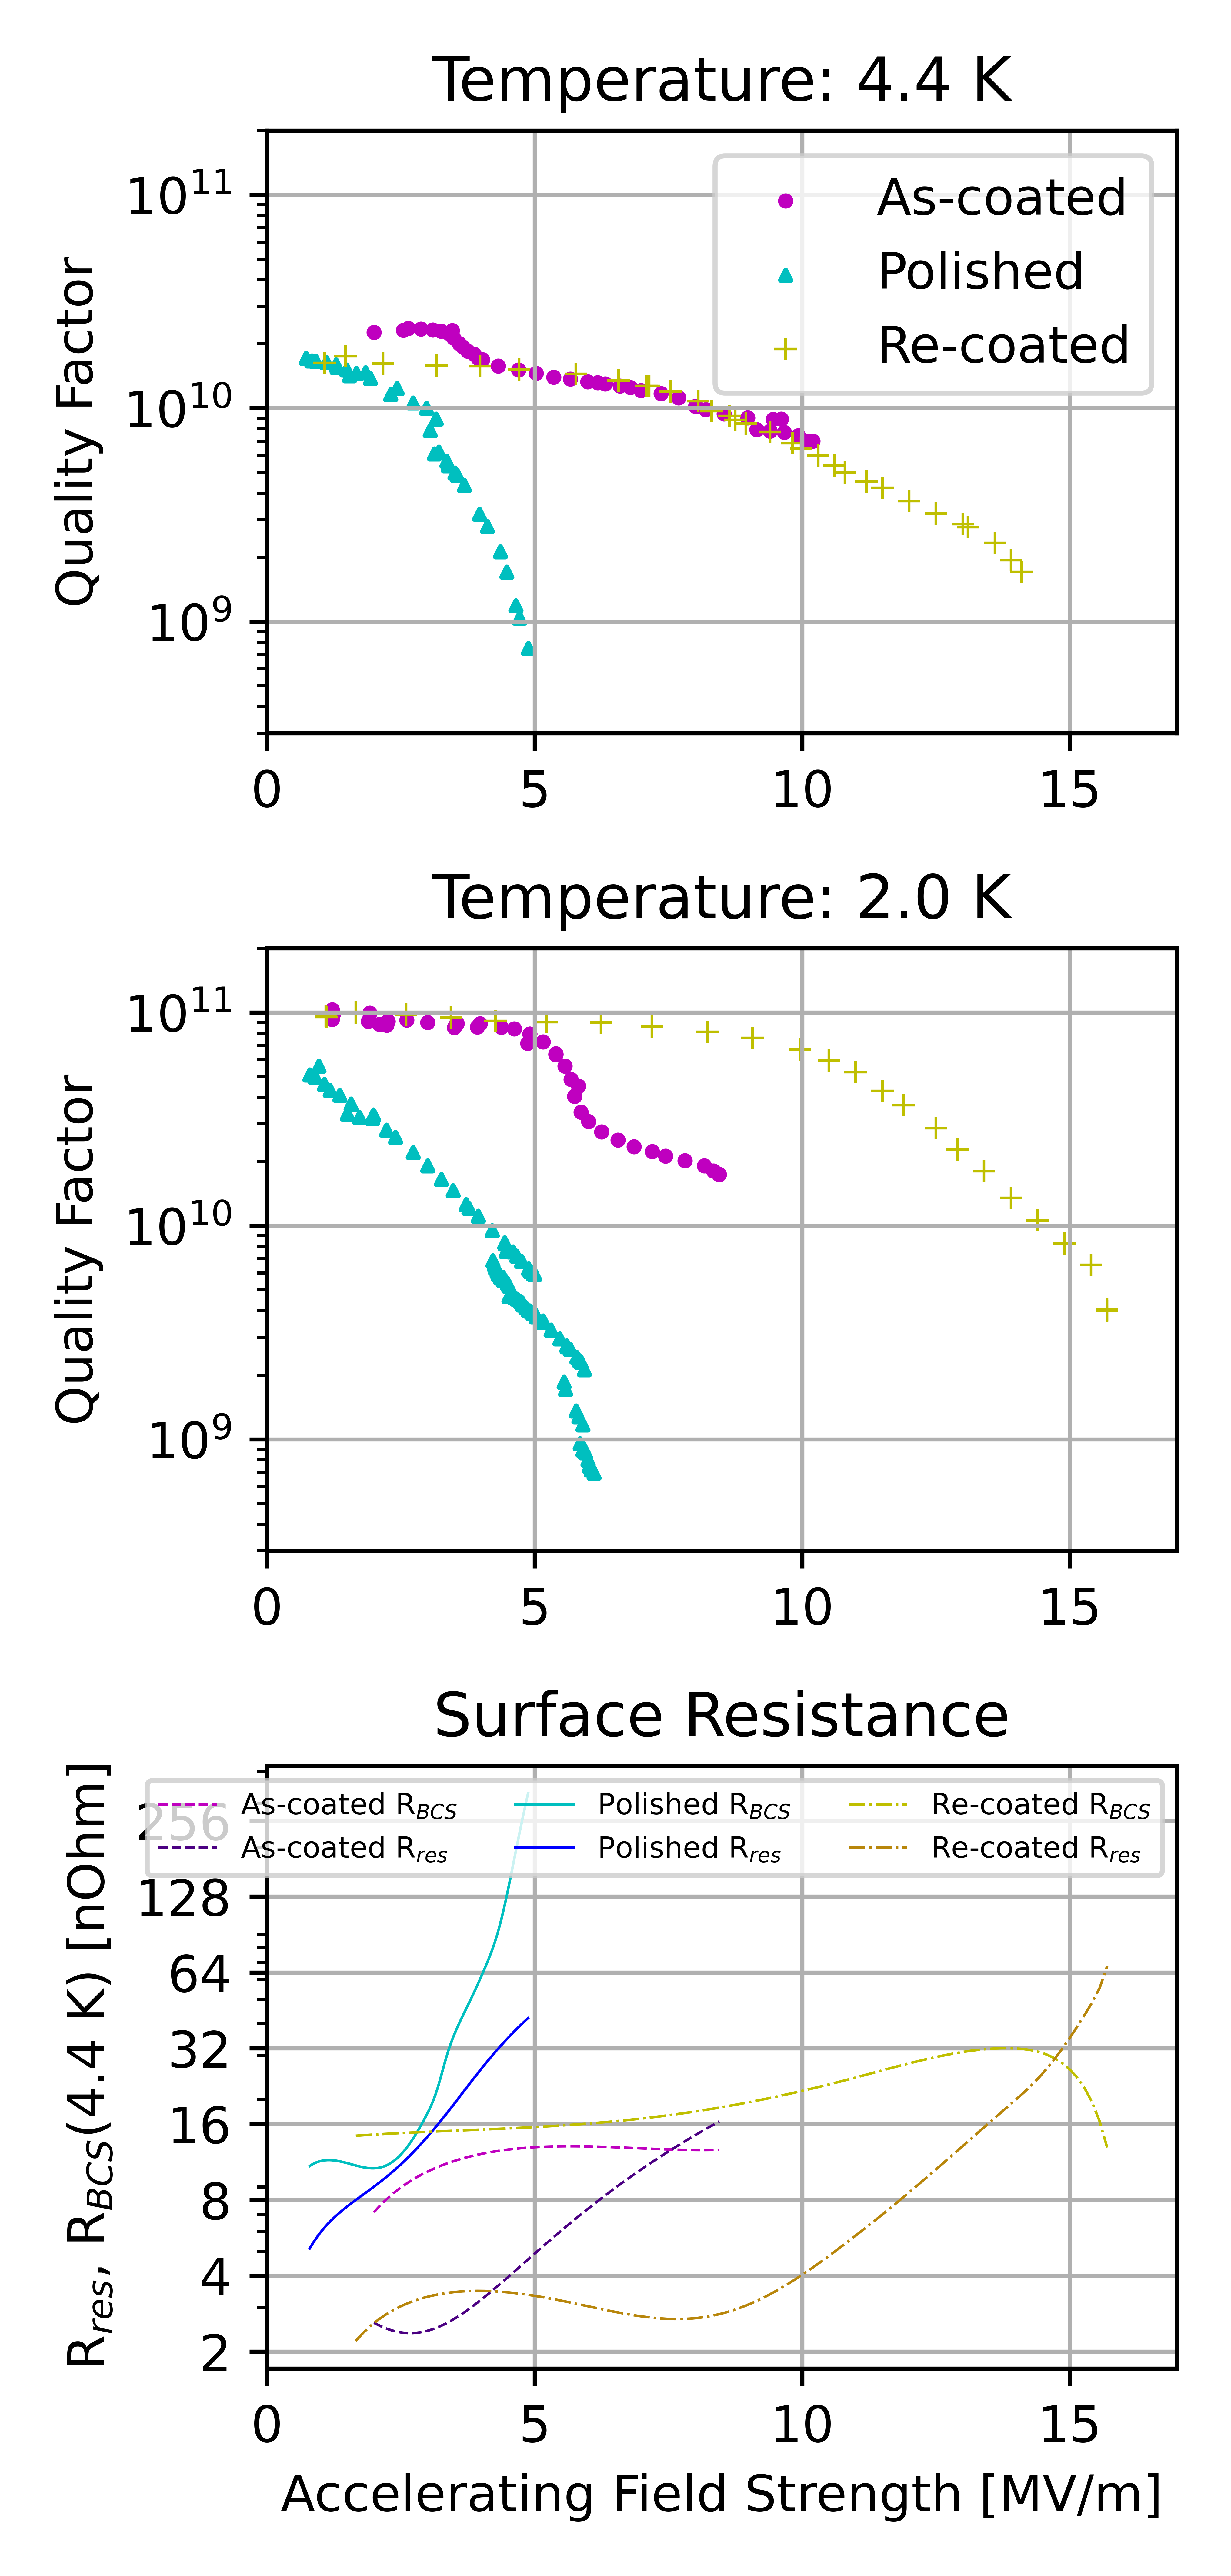
\includegraphics[width=\columnwidth]{../doc/figs/VTS_Test_Graph.png}%
                                \caption{\label{fig:vtstestgraph}The RF performance of the Nb\textsubscript{3}Sn-coated SRF cavity before and after mechanically polished and after a re-coating treatment.}
                            \end{figure}
                        \end{column}
                        \begin{column}{0.45\columnwidth}
                            Given that CBP was able to produce a smooth surface on Nb\textsubscript{3}Sn samples, the next step is to apply the polishing to a Nb\textsubscript{3}Sn cavity. A Nb\textsubscript{3}Sn-coated cavity was polished using the felt cube polishing media with a 50~nm alumina abrasive particle suspension, chosen to avoid the risk of silicon contamination in the coating furnace. The cavity was polished for 4~hours followed by high-pressure water rinsing and ultrasonic cleaning for 30~minutes to remove any residual abrasive material left by the polishing process. These parameters were chosen as a conservative estimate to minimize the possibility of removing the Nb\textsubscript{3}Sn film and allow for more material removal in the future while still providing a considerable improvement in surface roughness.
                        \end{column}
                    \end{columns}    
                    \begin{enumerate}
                        \item The Nb\textsubscript{3}Sn-coated cavity was polished using CBP leading to a shiny surface.
                        \item A re-coating procedure was applied to repair surface damage and subsurface defects at 1,000°C, using one third of the normal amount of tin and no SnCl\textsubscript{2}.
                        \item RF performance of the cavity was tested three times using the vertical test stand (VTS) at FNAL.
                        \item The as-coated performance was poor, with a maximum gradient of around 10MV/m and Q of 10\textsuperscript{10} at 4.4K.
                        \item After polishing, the cavity exhited Q-slope and the maximum gradient was only 5MV/m.
                        \item After the re-coating procedure, the Q-slope was ameliorated, and the maximum accelerating gradient increased to 15MV/m.
                        \item The quality factor of the cavity was also improved over the as-coated state at 2.0K, but not at 4.4~K.
                    \end{enumerate}
                    
                \end{block}
            \end{column}
        \end{columns}
    \end{frame}
\end{document}